\title{
  IoTデバイスに電源と時刻と例外を提供する RaspberryCom*PoTE の設計実装
  %% と使われなくなった情報コンセントの活用事例
}

\etitle{
  Design and Implemntasion of RaspberryCom*PoTE
}

\affiliate{Kanazawa}{金沢大学 総合メディア基盤センター\\
Kakuma-machi, Kanazawa, Ishikawa 920-1192, Japan}
\affiliate{USP}{ユニバーサル・シェル・プログラミング研究所}

\author{大野 浩之}{Hiroyuki Ohno}{Kanazawa}[hohno@staff.kanazawa-u.ac.jp]

%% ---------------------------------------------------------
%% 概要(90%)(0.75p タイトルと概要)
%% ---------------------------------------------------------

\begin{abstract}
IoTデバイスを長期間安定運用するには,安定した電源供給が必要である.
また,用途によっては遠隔からの強制再起動が可能が望まれる場合がある.
さらに,特に多数のIoTデバイスを運用する場合には,正確な時刻が必要となる場合がある.
そこで,IoTデバイスに対し,外部から電源と時刻と例外発生を安定して提供するしくみを設計し,これを {\tt RaspberryCom*PoTE}(ラズベリー・コンポート) と名付けた.
本報告では,大学の研究室程度の規模の室内環境での運用を前提とした{\tt Raspberry\-Com*PoTE}の設計実装とその運用について報告する.
\end{abstract}

\begin{jkeyword}
IoT, ものづくり, ものグラミング, Raspberry Pi, Arduino, POSIX, POSIX中心主義, 有線IoT
\end{jkeyword}


\begin{eabstract}
abstract, abstract, abstract, abstract, abstract, abstract, abstract, abstract, abstract, abstract,
\end{eabstract}

\begin{ekeyword}
IoT, Mono-gramming, Monogramming, Raspberry Pi, Arduino, POSIX, POSIX centrics approach, Wired IoT
\end{ekeyword}

\maketitle


\underline{(ここまでで0.75p)}\\

%% ---------------------------------------------------------
%%  1. はじめに(00%)(0.25p / 1.0)
%% ---------------------------------------------------------

\section{はじめに \small{\underline{(0.25p / 1.0)}}}
\label{sec:01introduction}

IoTデバイスを長期間安定運用するには,安定した電源供給が必要である.
そのための方法として,IoTデバイスの消費電力を極力小さくして,内蔵バッテリのバッテリの寿命を当該装置の想定設置期間より長くする方法がある.
この方法であれば,電池交換の必要はなくなり電源は安定的に供給される.ただし,現状ではこの方法ではIoTデバイスの消費電力は大きくはできない.
このため,センサを接続して計測結果を無線ネットワーク経由で母機となる機材に通知する用途では実用例があるが,アクチュエータを接続して母機からの指示にしたがって何かを動かす用途には適さない.
消費電流が大きい用途では太陽電池などで必要な電力を自給するといった方法もあるが,これも人間にとっては明るくても太陽電池にとっては十分な明るさではない室内のような環境には適さない.外部から電源を供給する従来の方法は引き続き有効な場面が多い.

電源供給方法の議論とは別に,遠隔からの強制再起動が可能だと望ましい場合がある.
さらに,特に多数のIoTデバイスを研究開発しつつ実際運用するような場合には,それぞれのIoTデバイスが保持する時刻が正しい時刻に同期している必要がある場合がある.
%%(※メモ:この文↑もう少し調整)

そこで,大学の研究室程度の規模の室内環境での運用を前提とした「IoTデバイスのために
電源\textgt{\textbf{(\underline{Po}wer)}} と
時刻\textgt{\textbf{(\underline{T}ime)}}と
例外\textgt{\textbf{(\underline{E}xception)}} を
外部から安定供給する
共通\textgt{\textbf{(\underline{Com}mon)}} の
複合的\textgt{\textbf{(\underline{Com}plex)}}な機構とそのための
構成要素\textgt{\textbf{(\underline{Com}ponent)}}
」を設計実装し,これを
%% \textgt{\textbf{Raspberry\underline{Com*PoTE}}}
{\tt Raspberry\underline{Com*PoTE}}
(ラズベリー・コンポート)と名付けて供用を開始した.

本報告では,{\tt Raspberry\-Com*PoTE}の設計実装について述べた,現時点での運用結果についても報告する.

%% ---------------------------------------------------------
%%  2. 背景(00%)0.75P / 1.75
%% ---------------------------------------------------------
\section{背景 \small{\underline{(0.75p / 1.75)}}}
\label{sec:02background}

著者の最近の興味は,大学の研究室のような規模の室内環境でIoTデバイスを長期に渡って安全安心かつ簡単に取り扱える環境の整備である.

これまでにも RaspberryGateや RaspberryGuardianを設計実装して,IoTデバイスのセキュリティを確保するためのセキュリティゲートウェイの構築と運用機構を実装したり\cite{hohno:RaspberryGate}\cite{hohno:RaspberryGuardian} ,
I2Cベースの近距離有線ネットワークを提案し室内環境でのIoTデバイスの運用環境を検討したり\cite{hohno:I2CwiredLAN-2017},
「ものグラミング」と名付けたIoT環境向けプログラミング手法を提案したりしてきた\cite{hohno:monogramming2}.

著者は,2017年に報告したI2Cベースの近距離有線ネットワークの運用経験を踏まえ,一部を簡素化した上で新たな機能を追加したしくみを検討した.
具体的には,2017年に提案した方式(以後「2017年方式」と呼ぶ)から長距離I2C通信機能を削除し,これに伴いI2Cバスから基準信号を発生する機能も削除した.
代わりに以下の機能を改良・強化あるいは追加し,簡単で使い勝手のよいしくみの実現を目指した.
%% なお、2017年に報告したI2Cベースの近距離有線ネットワークには特段の名前がついていないので,以後「2017年方式」と呼ぶ.

\begin{itemize}
\item (改良) 安定した電源供給
\item (強化) 例外(再起動、H/W割り込み)の通知
\item (新規) 環境情報(時刻等)の通知
\end{itemize}

なお,2017年方式には存在し,本研究では削除した長距離I2C通信機能については,その後通信方式を差動型に変更して距離の延長と安定を確保した(未発表).この成果は次の世代の {\tt Raspberry\-Com*PoTE} に取り込む予定である.これについては考察で言及する.

%% (※メモ:↑「考察で言及」してね)

%% (※メモ) これまでIOT環境関連では以下を実施してきた\\
%% \begin{itemize}
%% \item Raspbery Gate
%% \item Raspbery Guardian
%% \item ものぐらみんぐ
%% \item I2Cベースの近距離有線ネットワーク(2017年方式)
%% \end{itemize}

%% (※メモ) 前提となる現在の(自分の)研究環境\\

%% (※メモ) 現状、少なくとも現用の環境では室内に設置されたIOTデバイスには以下の需要がある\\
%% \begin{itemize}
%% \item (必須)安定した電源供給
%% \item (重要)例外状態通知(再起動、H/W割り込み)
%% \item (有用)時刻等の環境情報の通知
%% \end{itemize}

%% ---------------------------------------------------------
%%  3.関連研究(00%)0.75P / 2.5
%% ---------------------------------------------------------
\section{関連研究 \small{\underline{(0.75p / 2.5)}}}
\label{sec:03relatedworks}

本研究で提案する{\tt Raspberry\-Com*PoTE}に最も近いのは,著者が取り組んだ2017年方式である.
{\tt Raspberry\-Com*PoTE}は2017年方式の延長上にある.

2017年方式では8芯ケーブルを用い,そのうちの4芯で電源とI2Cバスを提供し,残りの4芯を2つ目のI2Cバスにしたり関連機能を付与したりするために付加的に用いる.{\tt Raspberry\-Com*PoTE}と比べると電源を供給するという考え方は同じであるが,{\tt Raspberry\-Com*PoTE}ではI2Cバスは提供していない.
I2Cバスを持たないため,I2Cバスのロックアップ回避・回復機能ももたない.
一方,両方式ともIoTデバイスに時刻情報を供給することは重要だと考えているが,2017年方式では基準時間信号と称する正確なクロックを提供しようとしているのに対して,{\tt Raspberry\-Com*PoTE}では時刻情報そのものを適切なタイミングで供給している.
また,{\tt Raspberry\-Com*PoTE}では時刻は「環境情報」の一つと位置づけており,時刻以外にも気温,湿度,気圧,明るさといったIoTデバイス群が設置された環境に関する情報を共有できる.
さらに,{\tt Raspberry\-Com*PoTE}では必須の機能として実現しているハードウェア割り込みやハードウェア・リセットは,2017年方式ではオプション機能と位置づけ1-Wireでの構成管理に委ねている.以上をまとめたのが表\ref{tb:T2017_vs_RaspberryComPoTE}である.


\begin{table}[h]
  \begin{center}
    \begin{tabular}{|l|c|c|l|} \hline
      機能 & 2017年方式 & 本方式 & 備考 \\
      \hline
      電源供給 & ○ & ○ &\\
      通信 & ○  & ー & I2Cバス\\
      基準クロック & ○ & ー &\\
      現在時刻 & ー & ○ &\\
      その他の情報 & ー & △&今後対応\\
      構成管理 & △ & ー & 1-Wire,非必須\\
      割り込み & ー & ○ &\\
      リセット & ー & ○ &\\
      \hline
    \end{tabular}
    \label{tb:T2017_vs_RaspberryComPoTE}
    \caption{2017方式との比較}
  \end{center}
\end{table}



%% (※メモ:↑続き書いてね!)

本研究は「有線IoT」と呼ばれる分野に属する.有線IoT分野では標準化が行われており,今後多くの注目が集まる分野だと予想できる.

%% https://businessnetwork.jp/Detail/tabid/65/artid/6561/Default.aspx

%% (※メモ:↑続き書いてね!)

通信用の配線を使い,通信しつつ電力を供給する方式としては PoE(PowerOverEthernet)が普及している.
PoEの基本機能は2003年に発効したIEEE 802.3afで規定されており,これに従えばカテゴリ5以上のUTPケーブルを使って電力を供給できる.
通常,電力送出側の機器は直流48Vで送電し,受電側は最大で約13Wの電力を取り出せる.

%% (※メモ:↑続き書いてね!)

PoEとは逆に,電力線を使い,電力を供給しつつ通信も行う方式としては PLC(PowerLineCommunication 電力線通信)が存在する.

%% https://www.ntt.co.jp/journal/0407/files/jn200407088.pdf

日本においては電力線に450kHz以下の帯域の信号を重畳して通信を行う方式がまず実用化され,その後 2006年には 2〜30MHzの帯域も利用できるようになった.
後者は高速電力線通信と呼んで前者と区別する場合がある.前者では9600bps程度,後者では100Mbpsを超える通信速度を提供する機器が実用化されている.

一方,本研究ではハードウェア割り込み信号やハードウェア・リセット信号を電源線に重畳するが,
その信号は数Hzあるいはそれ以下の速度で電源電圧を変動させる程度で実現できるので,PLC技術は参考にはなるがそのまま採用する必要は特にない.


PLCではないが,電力供給用途の直流電源線に信号を乗せて通信を行う方式には,鉄道模型分野で使われている DCC (Digital Command Control) がある.

DCCは...

%% (※メモ:↑続き書いてね!)

%% (※メモ) \\
%% \begin{itemize}
%% \item I2Cベースの近距離有線ネットワーク(2017年方式)
%% \item 有線IoT...
%% \item PoE...
%% \item PLC...
%% \item DCC...
%% \end{itemize}

%% ---------------------------------------------------------
%%  4. 設計と実装(00%)3P / 5.5
%% ---------------------------------------------------------
\section{設計と実装 \small{\underline{(3.0p / 5.5)}}}
\label{sec:04design_and_implementation}

本節では,{\tt Raspberry\-Com*PoTE}の設計方針を明らかにした後,実際の設計と実装について述べる.

%% ---------------------------------------------------------

\subsection{方針}

上述のように,電源供給・環境情報提供・例外状態通知3つの需要を満たす方法を設計実装するにあたり,以下の方針をとった

\begin{enumerate}
\item 配線に用いる線の数(配線材の芯数)はできるだけ少なくするなど,全体として簡素であることを重視する
\item 関連分野の既存の諸方式との互換性確保には固執しない
\item IoTデバイス同士,IoTデバイスと計測制御用コンピュータとの間で発生する実際の通信については積極的には提供しない
\item 日常の研究開発環境に投入して常時利用し,問題点があればフィードバックして改善する
\end{enumerate}

%% (※メモ:↑もう少し書けない?)

ここで,上記の第3項について補足する.

後述するように{\tt Raspberry\-Com*PoTE} では,環境情報の提供に RS-485 による有線通信を用いているので,{\tt Raspberry\-Com*PoTE} が提供する機能を用いて IoTデバイス同士やIoTデバイスと計測制御用コンピュータが相互に通信することは可能である.
しかし,このような機材間の通信は,頻度,通信量,実時間性への要求などが利用形態によって全く異なり,RS-485 で対応可能かは利用形態ごとに個別に検討する必要がある.
また,複数の異なる系が {\tt Raspberry\-Com*PoTE}を利用することは可能であるが,異なる系が一つの RS-485ネットワークを利用すると回線の利用を調停する必要が生じ,簡素に実現することはできない。
一方,現在では機材間の通信はWiFi, Bluetooth, その他の方法で実現できるのが普通であり,無理にRS-485の利用を強制する必要はない.そこで,機材間の実際の通信は {\tt Raspberry\-Com*PoTE} に含めないことにした.


この方針の下,{\tt Raspberry\-Com*PoTE} では4芯ケーブルを用いることとし,このうち2本で電源供給と例外状態通知を,残りの2本で環境情報の提供を実現することとした

ところで,拡張したI2Cバスを持つ2017年方式では8芯ケーブルを使うことを前提としている.
この8芯ケーブルを,今回提案する {\tt Raspberry\-Com*PoTE} で利用すると4芯が残る.
この残った4芯を用いれば,2017年方式の実装後に別途実装と評価を行った「差動方式のI2Cバス」(4芯必要)を導入できる.
機材間の通信を含めて全てを有線で構成したい場合は,通信速度がI2C通信の速度に拘束されてしまう問題があるが,この差動方式のI2Cバスの採用が有力である.
すなわち,8芯ケーブルを用いれば,2017年方式が提供していた有線通信と {\tt Raspberry\-Com*PoTE}とを融合させた別の方法を検討する余地がある.
このことについては考察にて言及する.

%% (※メモ:↑ちゃんと言及してね!)

%% ---------------------------------------------------------

\subsection{設計と実装}

上述の方針に基づいて設計実装した {\tt Raspberry\-Com*PoTE} の概要を図\ref{RaspberryComPoTE}に示す.

\begin{figure}[H]
\centering
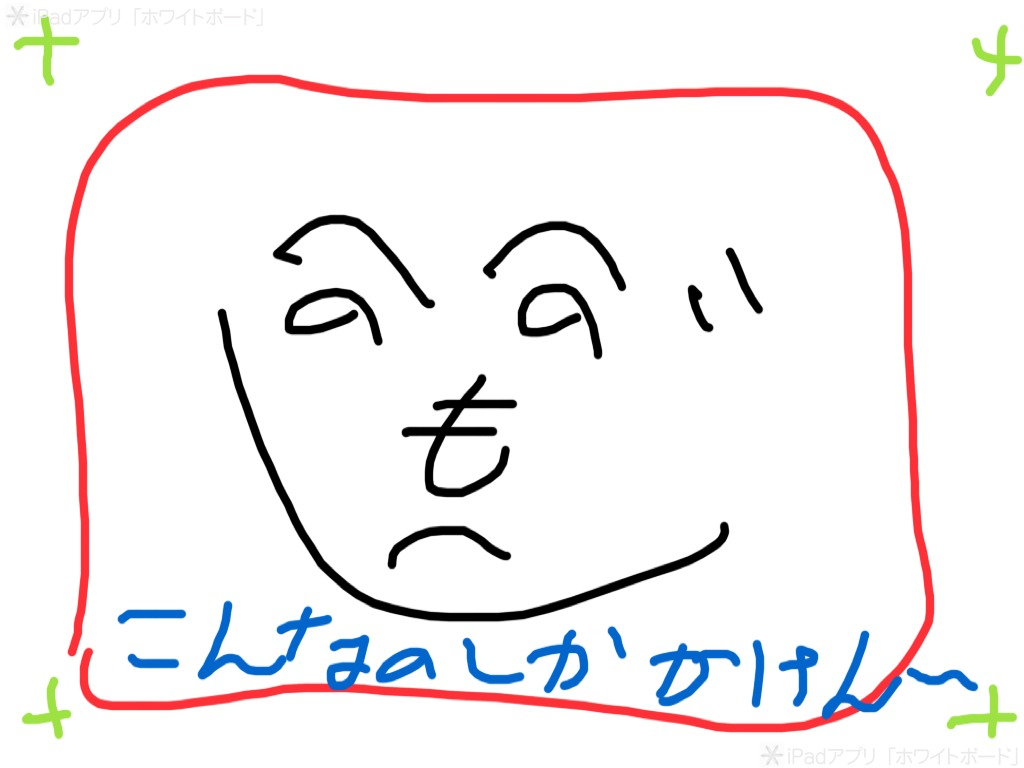
\includegraphics[width=5cm]{figspics/henoheno.jpeg}
\caption{{RaspberryComPoTE}全体構成図}
\label{RaspberryComPoTE}
\end{figure}

%% (※メモ:図)ここに全体構成図(図\ref{RaspberryComPoTE})を入れる

以下では上図に記された3つの系,すなわち電源供給系,例外状態通知系,環境情報提供系について述べる.


\subsubsection{電源供給系}

次項で述べるように{\tt Raspberry\-Com*PoTE}では,例外状態の発生を電源電圧の変動で表現する.
このため電源供給系は,単なる定電圧電源ではなく二つの異なる電圧間を必要なタイミングで遅延なく遷移する機能が必要になる.
2017年方式にも存在するこの機能は同方式と同様に非安定電源機能と名付けた.
非安定電源装置は外部からの指示で意図的に出力電圧を変動させ,
{\tt Raspberry\-Com*PoTE}を利用する各IoT機器に到達した時点では,4芯ケーブルを経由することで生じる電圧降下のため相応に低下した状態となる.
%% 同時に,二つの状態に対応した電位差はほぼそのまま伝わる.
しかし,機器ごとに必要な電源電圧は機器ごとに搭載する昇降圧型のレギュレータで生成sるため,
例外状態通知のための電源電圧の変動と4芯ケーブルを経由することで発生する電圧効果の影響は個別のIoT機器には及ばない.

現在の実装では電源供給系への入力電圧は,直流16V、出力電圧は通常時が DC 13.5V 前後,例外状態通知状態では 9V前後 としている.
また,各IoT機器側には4.5〜18Vの入力電圧を許容する3W級昇降圧型DC-DCコンバータを採用し,最終的には安定した DC5V 600mAを得ている.

例外を通知するための電源電圧の変動の速度は 数Hz程度であるため,通信としては超低速な部類になるが,
定電圧電源装置にスイッチングレギュレータを採用すると数Hzの速度で電圧を変化させることは難しい場合がある.
これはスイッチングレギュレータでは,二次側に容量の大きなコンデンサを取り付けるため,出力電源電圧を変更しても追従するためには秒単位の時間がかかるためである.
そこで今回は,スイッチングレギュレータより変換効率は劣るが設定電圧の変化への追随が早いシリーズ型の定電圧電源回路を採用しすることとし,LM338 5A可変レギュレータを用いて実装した.電源供給系の構成を図\ref{hono:RaspberryComPoTe-Po1}に示す.

%% http://www.ti.com/lit/ds/symlink/lm338.pdf

%% ,一次側はDC16.5V,二次側はDC13.5V(通常時)または9V(例外状態通知時)とした

\begin{figure}[H]
\centering
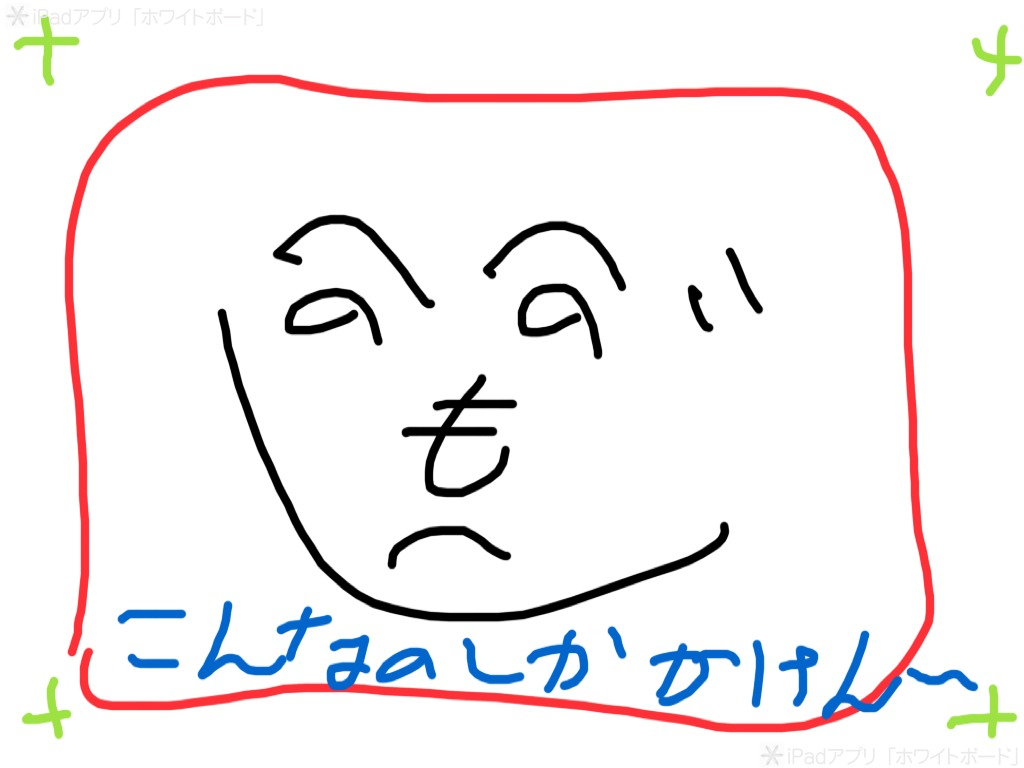
\includegraphics[width=5cm]{figspics/henoheno.jpeg}
\caption{電源供給系}
\label{hohno:RaspberryComPoTE-Po1}
\end{figure}

%% (※メモ:図)ここに電源出力系と各IoT機器側の受電系の図(図\ref{hohno:Po1})を入れる

%% (※メモ)過電圧遮断系も実装した

電源供給系の実装にあたっては,付加機能として過電流を検出した際に給電を停止し,警報を音と光で発報する機能も用意した.
通常,定電圧電源モジュールはシリーズ方式かスイッチング方式かに寄らず,設定以上の過電流が流れた場合一時的に給電を停止するか供給電圧を下げ,過電流状態が除去されるともとの給電を再開するのが普通である. {\tt Raspberry\-Com*PoTE}においても,最終的な長時間無停止無人運転時にはこのようなな挙動で問題ないが,現在はまだ試行錯誤を伴う運用があるため,過電流が流れた場合には給電を完全に停止するとともに光と音で警報を発し,
過電流の原因を除去したのちに手動で通電再開を指示しなければ給電を再開しないようにした.

この機構を追加したのは,意図せぬ誤接続誤接触で電源系がショートしたのにそれに気づくまでに時間を用意した経験が何度かあったためである.
これは,4芯ケーブルが長くなるとケーブルの抵抗成分が無視できない大きさになり,IoTデバイス側で電源まわりがショートしても非安定電源側ではたかだか5-10A程度の電流に留まるためである.このような場合,レギュレータは発熱はしても保護回路が働くまでに数10秒の時間を要したり,全く働かない.
つまり,過電流検出と電流制限をレギュレータに任せてしまうと,レギュレータの供給上限を上回る電流を流さない限り保護回路は働かないがケーブルの直流抵抗成分が供給上限以下の電流に留めてしまう.
たとえば今回用いた LM338 では5A以上の電流(場合によっては8A近い電流)が一定時間流れないと保護回路が働かない.
一方,開発中のIoTデバイスに誤電流が流れた場合,1Aかそれ以下の電流が流れても異常状態ということがあり得る.
しかし上述の理由によりこのような電流はLM338にとっては正常の範囲であって保護回路は働かない.
ここに,任意の値に設定できる過電流検出回路とそれに連携した給電停止回路を別途用意することで,異常状態とレギュレータの給電限界とを切り離せる.

このようにした上で,給電停止となったら音と光で警報を発するようにすれば,原因を除去するまでは給電停止と警報の発報が繰り返され,
不用意な通電による回路の損傷を回避できる.この回路の概要を図\ref{hohno:RaspberryComPoTE-Po2}に示す.

\begin{figure}[H]
\centering
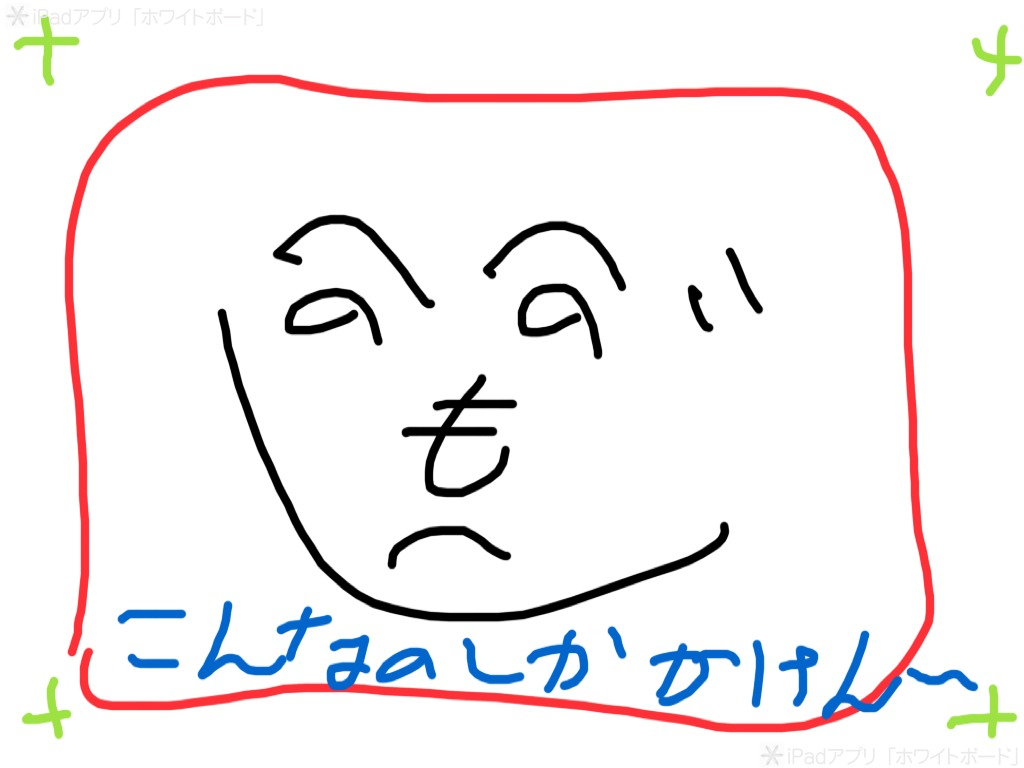
\includegraphics[width=5cm]{figspics/henoheno.jpeg}
\caption{過電流検出・警報}
\label{hohno:RaspberryComPoTE-Po2}
\end{figure}


%% 開発完了後の無停止運用においてはこのような手動操作を要求する機能は好ましくないが,開発完了まではこの機能を生かしておくことにした.

%% - - - - - - - - - - - - - - - - - - - - - - - - - - - - -

\subsubsection{例外状態通知系}

 {\tt Raspberry\-Com*PoTE}では,接続したIoTデバイスを一斉に再起動したり,主としてハードウェア割り込みを発生させるためのしくみを導入した.
 再起動(ハードウェア・リセット)やハードウェア割り込みの発生は,これらを受け入れる側にとっては例外的な状態であるため,これらを通知するしくみは「例外状態通知系」と呼んでいる.

 {\tt Raspberry\-Com*PoTE}では,現時点ではハードウェアリセット1種類とハードウェア割り込み1種類を提供している.これらの状態を通知するために,直上で述べた電源供給の非安定能を利用した.実装を簡単にするため,供給電圧が通常状態の約13.5Vから例外通知状態の約9Vへの降下を検出した時点でハードウェア割り込みを発生させ,それが一定時間(たとえば0.8秒)以上継続した場合にはさらにハードウェア・リセットを発生させる回路を用意した.
これにより電源電圧降下を2〜5Hzの速度で繰り返せばハードウェア割り込みは繰り返し発生し,ハードウェア割り込みハンドラ側でこの回数を数えることで,割り込み処理の挙動を順次変えることもできる.

\begin{figure}[H]
\centering
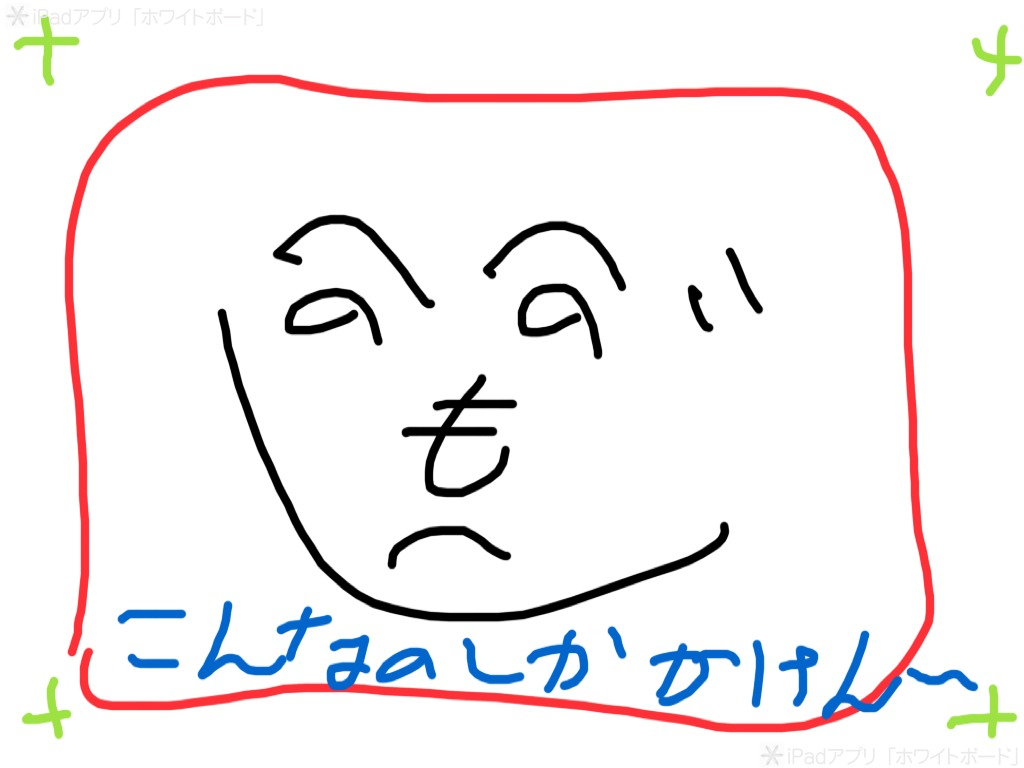
\includegraphics[width=5cm]{figspics/henoheno.jpeg}
\caption{例外状態通知系}
\label{hohno:RaspberryComPoTE-E}
\end{figure}


(※メモ:図)ここにリセット・割り込み回路の図(ブロック図(と回路図?))(図\ref{hohno:RaspberryComPoTE-E})を入れる


%% - - - - - - - - - - - - - - - - - - - - - - - - - - - - -

\subsubsection{環境情報提供系}


著者は,運用中のIoTデバイスの周囲の諸情報を環境情報と呼んでいる.
環境情報の筆頭は時刻情報である.時刻情報はIoTデバイスが何らかの情報を記録する際のタイムスタンプとなり,何らかの動作をする際のタイミングの基準となる.
時刻情報以外には気温や湿度を把握したい場合があるだろうし,用途によっては気圧や明るさ磁場電場なども必要かもしれない.

これらの情報は,IoTデバイスによっては,デバイス自体が自ら取得して利用できる場合があるが,小型のIoTデバイスではそのような機構が省かれることもある.
たとえば,時刻であれば実時間時計(RTC - Real Time Clock)を搭載するだけでは正確な現在時刻を取得するには不十分である.そのため時刻同期の仕組みが必要であるが,パソコンでよく利用される NTPサーバへアクセスしてNTPプロトコルを用いて時刻同期をするには,IoTデバイス側にTCP/IPプロトコルスタックを用意し,IP到達性を確保するための物理層とデータリンク層を用意しなければならない.IoTデバイスをできるだけ小規模に作ろうとした場合,NTPプロトコルによる時刻同期はソフトウェア領域を圧迫し新たなハードウェアの追加を必要とするなどオーバーヘッドが大きくなる.たとえば,Arduino UNOを用いた計測系を作る場合,Arduino UNO のプログラム領域はわずか 30kB程度でありここにTCP/IPプロトコルスタックに加え、DHCP, DNS, NTP などのサービスを書き加えると30kBの領域の可搬を消費してしまう.



(※メモ)引き続き書く

\subsubsubsection{環境情報提供サーバの時刻提供機能}

時刻情報の提供と取得は以下のように行う

まず時刻提供用の機材(環境情報サーバ)を用意する.必要なの以下の機能である.なおカッコ内には必要とな具体的な機能である.

\begin{itemize}
\item NTPサーバに到達できる機能(TCP/IPプロトコルスタック,IP到達性)
\item NTPサーバと時刻を同期を行い,内部のマイクロ秒カウンタの現在値とその時点でのUNIX秒(1970年1月1日0時0分0秒のUTCを0秒とする整数値)とのオフセットを求める機能(SNTPプロトコル)
\item RS-485回線に文字列を出力する機能(RS-485ドライバ)
\end{itemize}

この機能を使い,以下の手順で時刻情報をRS-485回線に送出する

\begin{enumerate}
\item 内部のマイクロ秒カウンタの下6桁がゼロになるタイミングの一定時間前(通常は100m秒程度)に改行文字を送出(これが「予報」となる)
\item 内部のマイクロ秒カウンタの下6桁がゼロになるタイミングでプリアンブルとなる ``T'' を送出
\item 続いてこのタイミングにおけるUTC値を送出る機能
\end{enumerate}

このため,環境情報サーバは ESP-8266 を用い Arduino開発環境上で C++言語を用いて実装した.

\begin{figure}[H]
\centering
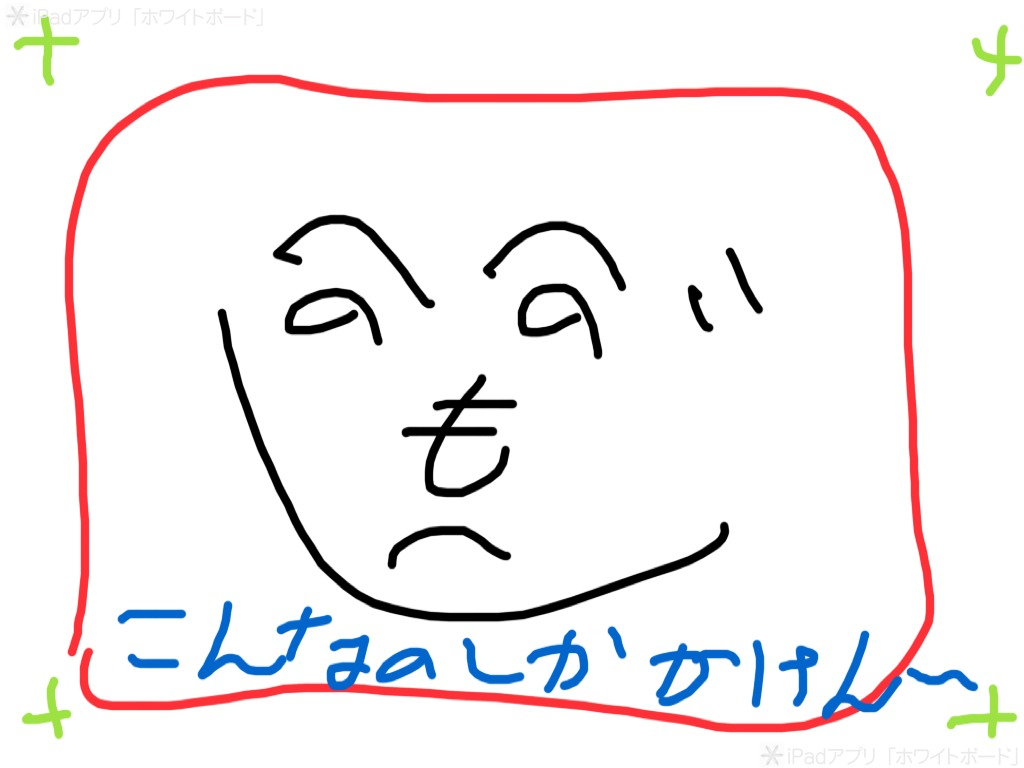
\includegraphics[width=5cm]{figspics/henoheno.jpeg}
\caption{環境情報提供系}
\label{hohno:RaspberryComPoTE-T}
\end{figure}

(※メモ:図)環境情報サーバの構成(図\ref{hohno:RaspberryComPoTE-T})

\subsubsubsection{環境情報提供サーバが提供する時刻との同期方法}

%% (※メモ)時刻情報の提供方法,受け取った側の同期方法

{\tt Raspberry\-Com*PoTE}を利用するIoTデバイスは RTCは搭載せずとも,Arduino UNOクラスの8ビットマイコンでも無理なく実現されている タイマ割り込みで更新するマイクロ秒カウンタが必須となる.そして以下の手順で,自らのマイクロ秒カウンタとUTCとのオフセットを決定する.

\begin{enumerate}
\item UARTから1バイト以上の読み出しが可能かを確認する.読み出せる文字がなければ他の作業に制御を移す.
\item もし1バイト以上の読み出しが可能なら1バイトずつ読み出し改行文字が現れるまで読み飛ばす.
\item 全て読んでも改行文字が現れなければ 1 に戻る
\item 改行文字が得られたら,一定時間以内(通常は100m秒程度)に次の文字が届き,それがプリアンブル(文字''T'')がくることを期待してビジーループで待機
\item 1バイ以上の呼び出しが可能になったらその時点でのマイクロ秒タイムカウンタの値 T0 を取得
\item プリアンブルがこなければ T0 を破棄して 1 に戻る.
\item プリアンブル以後の文字を取得できるだけ取得してそれがUNIX秒として妥当な文字列なければ T0 を破棄して 1に戻る
\item UNIX秒として妥当な文字列が取得できたらこの文字列を UNIX秒を示す整数値に変換する.5で取得した T0は,このUNIX秒に対応するマイクロ秒カウンタの値である.
\end{enumerate}

この方法には,時刻ずれを生じる要素として以下が考えられる.

\begin{enumerate}
\item 環境情報提供サーバのマイクロ秒カウンタから得られるUTCの推定値と実際のUTCのずれ(NTP時刻同期の誤差)
\item 環境情報提供サーバがプリアンブルを出力してから,IoTデバイスがUARTからプリアンブルを読み出すまでの時間
\item IoTデバイスが1文字読み出してからマイクロ秒カウンタの値 T0 を取得するまでの時間
\end{enumerate}

このうち 1 は通常は1ミリ秒より十分小さな値で数〜数10マイクロ秒に追い込める場合が多い.
2は、RS-485回線の通信速度が {\tt Raspberry\-Com*PoTE} が採用する 57600bps の場合,140μ秒程度かかるが,ゆらぎのない固定値とみなせる値である.
3は10マイクロ秒かそれより十分小さい以下であり,実験によってゆらぎのない固定値を取得可能である.
以上のことから {\tt Raspberry\-Com*PoTE} による時刻同期は1ミリ秒より十分小さい値に追い込めることがわかる.


\subsubsubsection{{\tt Raspberry\-Com*PoTE}における時刻同期を実現するスケッチ}

前目で述べた手順をArduino UNO用のクラスライブラリとして実装した.

(※メモ)SoftwareSerial や Serial1 を使った

(※メモ)どのくらいの大きさ?

\subsubsubsection{時刻以外の環境情報の提供と利用}


(※メモ)時刻以外の環境情報


%% ---------------------------------------------------------
%%  5. 評価(00%)0.75P / 6.25
%% ---------------------------------------------------------
\section{評価 \small{\underline{(0.75p / 6.25)}}}
\label{sec:05evaluation}

%% ---------------------------------------------------------

\subsection{評価方法}

(※メモ) 評価方法を提示する\\

\subsubsection{電源供給系}

(※メモ) 電源電圧の遷移が想定の速度でできるかを確認する\\

%% - - - - - - - - - - - - - - - - - - - - - - - - - - - - -

\subsubsection{例外状態通知系}

(※メモ) 電源電圧の遷移によってハードウェア割り込みとハードウェア・リセットができるか確認する.ハードウェア割り込みが一定の速度で繰り返された場合,ハードウェア・リセットを起こすことなくハードウェア割り込みを繰り返せるかを確認する

%% - - - - - - - - - - - - - - - - - - - - - - - - - - - - -

\subsubsection{環境情報提供系}

(※メモ) 今回の評価は時刻同期に限定する. {\tt Raspberry\-Com*PoTE}にArduino UNOを接続して時刻同期させて上で毎正秒ごとに正秒パルスを発生させる.同時にGPS受信機からも正秒パルス出力し両者の時差をマイクロ秒単位で計測する


%% ---------------------------------------------------------

\subsection{評価結果}

(※メモ) 評価結果を提示する\\

\subsubsection{電源供給系}


%% - - - - - - - - - - - - - - - - - - - - - - - - - - - - -

\subsubsection{例外状態通知系}

%% - - - - - - - - - - - - - - - - - - - - - - - - - - - - -

\subsubsection{環境情報提供系}


%% ---------------------------------------------------------
%%  6. 考察(00%)0.75P / 7.0
%% ---------------------------------------------------------
\section{考察 \small{\underline{(0.75p / 7.0)}}}
\label{sec:06discussion}

(※メモ) 他の方法との比較
\\


%% ---------------------------------------------------------
%% 7. 今後の展開(00%)0.5P / 7.5
%% ---------------------------------------------------------
\section{今後の展開 \small{\underline{(0.5p / 7.5)}}}
\label{sec:07nextstep}

今後の展開については以下の3つの方向がある

一つ目は,現在の {\tt Raspberry\-Com*PoTE} の量的拡張で,著者の研究室周辺で利用可能箇所を増やすとともに,著者の研究グループ内外への展開も行いたい.

(※メモ)

二つ目は,現在の {\tt Raspberry\-Com*PoTE} の質的拡張で,距離と安定性を増したI2Cベースの近距有線ネットワーク機能の追加を行う.


(※メモ)

三つ目は,

(※メモ)検討中


%% ---------------------------------------------------------
%% 8. おわりに(00%)(0.25P / 7.75
%% ---------------------------------------------------------
\section{おわりに \small{\underline{(0.25p / 7.25)}}}
\label{sec:07conclusion}

本研究では...


(※メモ)検討中

%% ---------------------------------------------------------
%%  謝辞(0%)(これ以降で 0.25p / 8.0)
%% ---------------------------------------------------------

\underline{(これ以降で 0.25p / 8.0)}\\

\begin{acknowledgment}
  本研究を遂行するにあたり,カナダ国ノバスコシア州立ダルハウジー大学コンピュータサイエンス学部の Prof. Sampalli および同教授の研究室の学生からは,「ものグラミング」の有効性について検討する際に多くの示唆を得た.この経験が,{\tt Raspberry\-Com*PoTE}の開発を後押しした.
  また,ユニバーサル・シェル・プログラミング研究所の當仲寛哲所長をはじめとする同社の研究部門の方々との議論も有益であった.ここに記して感謝したい.
\end{acknowledgment}


%% ---------------------------------------------------------

%% \newpage

\begin{thebibliography}{2}

%% 01
\bibitem{hohno:monogramming1}
  大野,森,北口,中村,松浦,石山,當仲,ものづくりのための「ものグラミング」と実践的教育環境の構築,DICOMO2016,1335-1340, 2016-07.

%% 02
\bibitem{misc:POSIXdocs1}
  What is POSIX?,The Open Group (オンライン),
  \urlj{https://collaboration.opengroup.org/external/pasc.org/plato/}
  \refdatej{2019-02-04}

%% 03
\bibitem{matsuura:POSIXcentrics}
  松浦智之,大野浩之,當仲寛哲,ソフトウェアの高い互換性と長い持続性を目指すPOSIX中心主義プログラミング,デジタルプラクティス 8(4),352-360,2017-10-15.

%% 04
\bibitem{misc:WSL_arch_overview}
  Seth Juarez,Windows Subsystem for Linux: Architectural Overview (オンライン),
  \urlj{https://channel9.msdn.com/Blogs/Seth-Juarez/Windows-Subsystem-for-Linux-Architectural-Overview}
  \refdatej{2019-05-22}

%% 05
\bibitem{misc:firmata}
  Firmata Library
  \urlj{https://www.arduino.cc/en/Reference/Firmata}
  \refdatej{2019-05-22}

%% 06
\bibitem{misc:kotoriotoko}
  秘密結社シェルショッカー日本支部,恐怖!小鳥男 (オンライン),
  \urlj{https://github.com/ShellShoccar-jpn/kotoriotoko}
  \refdatej{2019-02-04}

%% 07
\bibitem{hohno:RaspberryGate}
  ※大野浩之,RaspberryGate,情報処理学会, ...

%% 08
\bibitem{hohno:RaspberryGuardian}
  ※大野浩之,RaspberryGuardian,情報処理学会, ...

%% 09
\bibitem{hohno:I2CwiredLAN-2017}
  ※大野浩之,データ通信機能に電源供給・回線復旧・基準信号供給機能を加えたI2Cベースの近距離有線ネットワークの提案,情報処理学会研究会報告,Vol.2017-IOT-38,No.12,2017-06-24.

%% 10
\bibitem{hohno:monogramming2}
  ※大野浩之,森祥寛,松浦智之,  ものグラミング2 --諸機能の選択と集中を徹底したPOSIX 中心主義に基づくIoT開発方式の提案--, 情報処理学会研究会報告,Vol.2019-IOT-46,No.00,2019-06-14.

\end{thebibliography}

%% ---------------------------------------------------------
